\icode{E-MCH-SI-L3-261026-001}
如图所示，在斜面顶端先后水平抛出同一小球，第一次小球落到斜面中点，第二次小球落到斜面底端，从抛出到落至斜面上（忽略空气阻力），下列说法正确的是\paren[]

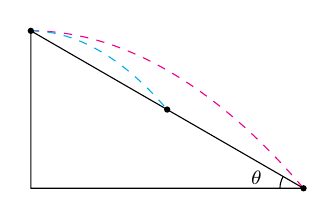
\begin{tikzpicture}[font=\scriptsize]
	\draw (0,0)--(150:4)|-(0,0);
	\draw[dashed,magenta] (150:4) parabola bend(150:4)(0,0);
	\draw[dashed,cyan] (150:4) parabola bend(150:4)(150:2);
	\draw (-.3,0) arc (180:150:.3);
	\node at(-.6,.14){ \(\theta\)};
	\foreach \c in {(0,0),(150:4),(150:2)}
		\fill \c circle(.04);
\end{tikzpicture}
\begin{choices}
	\item 两次小球运动时间之比\(t_1:t_2=\sqrt{2}:1\)
	\item 两次小球运动时间之比\(t_1:t_2=1:2\)
	\item 两次小球抛出时初速度之比\(v_{01}:v_{02}=1:\sqrt{2}\)
	\item 两次小球抛出时初速度之比\(v_{01}:v_{02}=1:2\)
\end{choices}
\begin{answer}
	C\qquad 提示：
\end{answer}